\documentclass[]{article}
\usepackage{lmodern}
\usepackage{amssymb,amsmath}
\usepackage{ifxetex,ifluatex}
\usepackage{fixltx2e} % provides \textsubscript
\ifnum 0\ifxetex 1\fi\ifluatex 1\fi=0 % if pdftex
  \usepackage[T1]{fontenc}
  \usepackage[utf8]{inputenc}
\else % if luatex or xelatex
  \ifxetex
    \usepackage{mathspec}
  \else
    \usepackage{fontspec}
  \fi
  \defaultfontfeatures{Ligatures=TeX,Scale=MatchLowercase}
\fi
% use upquote if available, for straight quotes in verbatim environments
\IfFileExists{upquote.sty}{\usepackage{upquote}}{}
% use microtype if available
\IfFileExists{microtype.sty}{%
\usepackage{microtype}
\UseMicrotypeSet[protrusion]{basicmath} % disable protrusion for tt fonts
}{}
\usepackage[margin=1in]{geometry}
\usepackage{hyperref}
\hypersetup{unicode=true,
            pdftitle={How to use the mybcart package},
            pdfauthor={Bruna Wundervald},
            pdfborder={0 0 0},
            breaklinks=true}
\urlstyle{same}  % don't use monospace font for urls
\usepackage{color}
\usepackage{fancyvrb}
\newcommand{\VerbBar}{|}
\newcommand{\VERB}{\Verb[commandchars=\\\{\}]}
\DefineVerbatimEnvironment{Highlighting}{Verbatim}{commandchars=\\\{\}}
% Add ',fontsize=\small' for more characters per line
\usepackage{framed}
\definecolor{shadecolor}{RGB}{248,248,248}
\newenvironment{Shaded}{\begin{snugshade}}{\end{snugshade}}
\newcommand{\AlertTok}[1]{\textcolor[rgb]{0.94,0.16,0.16}{#1}}
\newcommand{\AnnotationTok}[1]{\textcolor[rgb]{0.56,0.35,0.01}{\textbf{\textit{#1}}}}
\newcommand{\AttributeTok}[1]{\textcolor[rgb]{0.77,0.63,0.00}{#1}}
\newcommand{\BaseNTok}[1]{\textcolor[rgb]{0.00,0.00,0.81}{#1}}
\newcommand{\BuiltInTok}[1]{#1}
\newcommand{\CharTok}[1]{\textcolor[rgb]{0.31,0.60,0.02}{#1}}
\newcommand{\CommentTok}[1]{\textcolor[rgb]{0.56,0.35,0.01}{\textit{#1}}}
\newcommand{\CommentVarTok}[1]{\textcolor[rgb]{0.56,0.35,0.01}{\textbf{\textit{#1}}}}
\newcommand{\ConstantTok}[1]{\textcolor[rgb]{0.00,0.00,0.00}{#1}}
\newcommand{\ControlFlowTok}[1]{\textcolor[rgb]{0.13,0.29,0.53}{\textbf{#1}}}
\newcommand{\DataTypeTok}[1]{\textcolor[rgb]{0.13,0.29,0.53}{#1}}
\newcommand{\DecValTok}[1]{\textcolor[rgb]{0.00,0.00,0.81}{#1}}
\newcommand{\DocumentationTok}[1]{\textcolor[rgb]{0.56,0.35,0.01}{\textbf{\textit{#1}}}}
\newcommand{\ErrorTok}[1]{\textcolor[rgb]{0.64,0.00,0.00}{\textbf{#1}}}
\newcommand{\ExtensionTok}[1]{#1}
\newcommand{\FloatTok}[1]{\textcolor[rgb]{0.00,0.00,0.81}{#1}}
\newcommand{\FunctionTok}[1]{\textcolor[rgb]{0.00,0.00,0.00}{#1}}
\newcommand{\ImportTok}[1]{#1}
\newcommand{\InformationTok}[1]{\textcolor[rgb]{0.56,0.35,0.01}{\textbf{\textit{#1}}}}
\newcommand{\KeywordTok}[1]{\textcolor[rgb]{0.13,0.29,0.53}{\textbf{#1}}}
\newcommand{\NormalTok}[1]{#1}
\newcommand{\OperatorTok}[1]{\textcolor[rgb]{0.81,0.36,0.00}{\textbf{#1}}}
\newcommand{\OtherTok}[1]{\textcolor[rgb]{0.56,0.35,0.01}{#1}}
\newcommand{\PreprocessorTok}[1]{\textcolor[rgb]{0.56,0.35,0.01}{\textit{#1}}}
\newcommand{\RegionMarkerTok}[1]{#1}
\newcommand{\SpecialCharTok}[1]{\textcolor[rgb]{0.00,0.00,0.00}{#1}}
\newcommand{\SpecialStringTok}[1]{\textcolor[rgb]{0.31,0.60,0.02}{#1}}
\newcommand{\StringTok}[1]{\textcolor[rgb]{0.31,0.60,0.02}{#1}}
\newcommand{\VariableTok}[1]{\textcolor[rgb]{0.00,0.00,0.00}{#1}}
\newcommand{\VerbatimStringTok}[1]{\textcolor[rgb]{0.31,0.60,0.02}{#1}}
\newcommand{\WarningTok}[1]{\textcolor[rgb]{0.56,0.35,0.01}{\textbf{\textit{#1}}}}
\usepackage{graphicx,grffile}
\makeatletter
\def\maxwidth{\ifdim\Gin@nat@width>\linewidth\linewidth\else\Gin@nat@width\fi}
\def\maxheight{\ifdim\Gin@nat@height>\textheight\textheight\else\Gin@nat@height\fi}
\makeatother
% Scale images if necessary, so that they will not overflow the page
% margins by default, and it is still possible to overwrite the defaults
% using explicit options in \includegraphics[width, height, ...]{}
\setkeys{Gin}{width=\maxwidth,height=\maxheight,keepaspectratio}
\IfFileExists{parskip.sty}{%
\usepackage{parskip}
}{% else
\setlength{\parindent}{0pt}
\setlength{\parskip}{6pt plus 2pt minus 1pt}
}
\setlength{\emergencystretch}{3em}  % prevent overfull lines
\providecommand{\tightlist}{%
  \setlength{\itemsep}{0pt}\setlength{\parskip}{0pt}}
\setcounter{secnumdepth}{0}
% Redefines (sub)paragraphs to behave more like sections
\ifx\paragraph\undefined\else
\let\oldparagraph\paragraph
\renewcommand{\paragraph}[1]{\oldparagraph{#1}\mbox{}}
\fi
\ifx\subparagraph\undefined\else
\let\oldsubparagraph\subparagraph
\renewcommand{\subparagraph}[1]{\oldsubparagraph{#1}\mbox{}}
\fi

%%% Use protect on footnotes to avoid problems with footnotes in titles
\let\rmarkdownfootnote\footnote%
\def\footnote{\protect\rmarkdownfootnote}

%%% Change title format to be more compact
\usepackage{titling}

% Create subtitle command for use in maketitle
\newcommand{\subtitle}[1]{
  \posttitle{
    \begin{center}\large#1\end{center}
    }
}

\setlength{\droptitle}{-2em}

  \title{How to use the \texttt{mybcart} package}
    \pretitle{\vspace{\droptitle}\centering\huge}
  \posttitle{\par}
    \author{Bruna Wundervald}
    \preauthor{\centering\large\emph}
  \postauthor{\par}
      \predate{\centering\large\emph}
  \postdate{\par}
    \date{March, 2019}

\usepackage{float}

\begin{document}
\maketitle

The \texttt{mybcart} package is a very slow implementation of the
Bayesian CART model, made mostly with functions of the
\texttt{tidyverse} collection of packages. The package can be installed
from GitHub with:

\begin{Shaded}
\begin{Highlighting}[]
\NormalTok{devtools}\OperatorTok{::}\KeywordTok{install_github}\NormalTok{(}\StringTok{"brunaw/my_BART"}\NormalTok{, }\DataTypeTok{subdir =} \StringTok{"package/mybcart"}\NormalTok{)}
\end{Highlighting}
\end{Shaded}

After that, a list of the available functions can be obtained with:

\begin{Shaded}
\begin{Highlighting}[]
\KeywordTok{library}\NormalTok{(mybcart)}
\KeywordTok{ls}\NormalTok{(}\StringTok{"package:mybcart"}\NormalTok{)}
\end{Highlighting}
\end{Shaded}

\begin{verbatim}
##  [1] "%>%"                    "bcart"                 
##  [3] "friedman_data"          "lk_ratio_grow"         
##  [5] "lk_ratio_prune"         "p_rule"                
##  [7] "predict_bcart"          "ratio_grow"            
##  [9] "ratio_prune"            "structure_ratio_grow"  
## [11] "structure_ratio_prune"  "transition_ratio_grow" 
## [13] "transition_ratio_prune"
\end{verbatim}

\hypertarget{brief-description-of-the-functions}{%
\subsection{Brief description of the
functions}\label{brief-description-of-the-functions}}

There are 11 functions in the package (besides the
\texttt{\%\textgreater{}\%} and the Friedman data), that can be
described as:

\begin{itemize}
\tightlist
\item
  \texttt{bcart}: a function that receives a formula, the data and the
  number of iterations to build the model, and depends on:

  \begin{itemize}
  \tightlist
  \item
    \texttt{lk\_ratio\_grow}: Calculates the likelihood ratio of a grow
    step;
  \item
    \texttt{lk\_ratio\_prune}: Calculates the likelihood ratio of a
    prune step;
  \item
    \texttt{structure\_ratio\_grow}: Calculates the tree structure ratio
    of a grow step;
  \item
    \texttt{structure\_ratio\_prune}: Calculates the tree structure
    ratio of a prune step;
  \item
    \texttt{transition\_ratio\_grow}: Calculates the transition ratio of
    a grow step;
  \item
    \texttt{transition\_ratio\_prune}: Calculates the transition ratio
    of a prune step;
  \item
    \texttt{ratio\_grow}: Combines the tree ratios of a grow step, to
    calculate the final acceptance value for the MCMC;
  \item
    \texttt{ratio\_prune}: Combines the tree ratios of a prune step, to
    calculate the final acceptance value for the MCMC;
  \item
    \texttt{p\_rule}: A function that selects the splitting rule in a
    grow step, given a variable uniformly selected.
  \end{itemize}
\item
  \texttt{predict\_bcart}: A function that performs the prediction for a
  \texttt{bcart} model, by receiveing the model and the new data.
\end{itemize}

More details about each function can be found in their documentation
inside the package, as well as the details for the ratios and the model
should be found in the maths file. The \texttt{bcart} function will
return a list containing:

\begin{itemize}
\tightlist
\item
  \texttt{sigma\_2}: The posterior values for \(\sigma^2_{y}\);
\item
  \texttt{errors}: The sum of the squared residuals calculated for each
  iteration of the model;
\item
  \texttt{final\_tree}: The final tree;
\item
  \texttt{ratios}: The calculated ratios in each step;
\item
  \texttt{samp\_unif}: The uniform values sampled to used in the MCMC;
\item
  \texttt{nodes}: The nodes, which were grown or pruned, used in each
  iteration of the model.
\item
  \texttt{action\_taken}: The action (prune, grow or nothing) taken in
  each iteration.
\item
  \texttt{results}: The order in which the growing happened for the
  final tree;
\item
  \texttt{mu}: The values for \(\mathbf{\mu}\) for the final tree, used
  in the prediction function.
\item
  \texttt{model\_formula}: The model formula, used in the prediction
  function.
\end{itemize}

\hypertarget{the-friedman-data}{%
\subsection{The Friedman data}\label{the-friedman-data}}

The package also contains some data to be used with the model. The data
was simulated using the model equation proposed in (Friedman (1991)). We
simulated a response variable \(Y\) and its relationship to a matrix of
predictors \(\mathbf{X}\) as

\begin{equation}
y_i = 10 sin(\pi x_{i1} x_{i2}) + 20 (x_{i3} -
0.5)^{2} + 10 x_{i4} + 5 x_{i5} +
 \epsilon_i, \thinspace
\epsilon_i \stackrel{iid}\sim N(0, \sigma^2),
\end{equation}

where \(\mathbf{X} \in [0, 1]\), meaning that the predictors were
randomly drawn from a standard Uniform distribution.

\hypertarget{how-to-use-it}{%
\subsection{How to use it}\label{how-to-use-it}}

The following code show how to actually use the functions, starting by
gathering the data, running the model and checking it, and using the
prediction function.

\begin{Shaded}
\begin{Highlighting}[]
\KeywordTok{library}\NormalTok{(tidyverse)}

\CommentTok{# Gathering the data and separating in train and test }
\NormalTok{data <-}\StringTok{ }\NormalTok{mybcart}\OperatorTok{::}\NormalTok{friedman_data }\OperatorTok\StringTok{ }
\StringTok{  }\KeywordTok{mutate}\NormalTok{(}\DataTypeTok{set =} \KeywordTok{ifelse}\NormalTok{(}\KeywordTok{runif}\NormalTok{(}\KeywordTok{nrow}\NormalTok{(.)) }\OperatorTok{>}\StringTok{ }\FloatTok{0.8}\NormalTok{, }\StringTok{"test"}\NormalTok{, }\StringTok{"train"}\NormalTok{))}

\NormalTok{train <-}\StringTok{ }\NormalTok{data }\OperatorTok\StringTok{ }\KeywordTok{filter}\NormalTok{(set }\OperatorTok{==}\StringTok{ "train"}\NormalTok{) }\OperatorTok\StringTok{ }\KeywordTok{select}\NormalTok{(}\OperatorTok{-}\NormalTok{set)}

\CommentTok{# Running the model}
\NormalTok{bcart_model <-}\StringTok{ }\NormalTok{mybcart}\OperatorTok{::}\KeywordTok{bcart}\NormalTok{(}\DataTypeTok{formula =}\NormalTok{ y }\OperatorTok{~}\StringTok{ }\NormalTok{., }\DataTypeTok{data =}\NormalTok{ train, }\DataTypeTok{iter =} \DecValTok{200}\NormalTok{)}
\end{Highlighting}
\end{Shaded}

\begin{verbatim}
## 
## # ----------------------------------------------------------  
## The tree has finished growing, with a final error 
## of: 405.5122 and a final posterior variance of: 0.499368 
## The minimum node depth is 2 and the maximum is  7 
## # ----------------------------------------------------------
\end{verbatim}

\begin{Shaded}
\begin{Highlighting}[]
\KeywordTok{str}\NormalTok{(bcart_model)}
\end{Highlighting}
\end{Shaded}

\begin{verbatim}
## List of 10
##  $ sigma_2      : num [1:201] 0.0747 0.9835 1.0002 0.8589 0.9493 ...
##  $ errors       : num [1:200] 797 797 688 688 687 ...
##  $ final_tree   :'data.frame':   798 obs. of  11 variables:
##   ..$ X1        : num [1:798] 0.7699 0.3034 0.6182 0.0432 0.8202 ...
##   ..$ X2        : num [1:798] 0.3015 0.705 0.1747 0.5511 0.0599 ...
##   ..$ X3        : num [1:798] 0.948 0.681 0.877 0.839 0.478 ...
##   ..$ X4        : num [1:798] 0.975 0.799 0.606 0.528 0.677 ...
##   ..$ X5        : num [1:798] 0.214 0.805 0.179 0.337 0.176 ...
##   ..$ y         : num [1:798] 1.881 1.016 -0.116 -0.942 -1.131 ...
##   ..$ node      : chr [1:798] "root X2 left X5 right X4 left X1 left X2 right" "root X2 left X5 left X4 right X1 right" "root X2 right X4 right X2 left" "root X2 left X5 right X4 left X1 right" ...
##   ..$ parent    : chr [1:798] "root X2 left X5 right X4 left X1 left" "root X2 left X5 left X4 right" "root X2 right X4 right" "root X2 left X5 right X4 left" ...
##   ..$ d         : num [1:798] 5 4 3 4 3 3 6 4 6 4 ...
##   ..$ node_index: num [1:798] 13 9 17 14 17 15 7 1 10 14 ...
##   ..$ criteria  : chr [1:798] "no split" "no split" "no split" "no split" ...
##  $ ratios       : num [1:200] NA 4.67e-06 1.00 1.01e-08 1.01e-10 ...
##  $ samp_unif    : num [1:200] NA 0.5123 0.5334 0.0217 0.2781 ...
##  $ nodes        : chr [1:200] NA "root" "root" "root X2 right" ...
##  $ action_taken : chr [1:200] NA "grow" "grow" "grow" ...
##  $ results      :'data.frame':   17 obs. of  3 variables:
##   ..$ node: chr [1:17] "root" "root X2 left" "root X2 right" "root X2 left X5 left" ...
##   ..$ var : chr [1:17] "X2" "X5" "X4" "X4" ...
##   ..$ rule: num [1:17] 0.265 0.617 0.813 0.836 0.336 ...
##  $ mu           : num [1:18] 1.3205 1.6576 1.8571 0.8152 -0.0779 ...
##  $ model_formula:Class 'formula'  language y ~ . - 1
##   .. ..- attr(*, ".Environment")=<environment: 0x7fea12610f90>
\end{verbatim}

\begin{Shaded}
\begin{Highlighting}[]
\CommentTok{# Checking some results of the model}
\KeywordTok{library}\NormalTok{(patchwork)}
\NormalTok{p1 <-}\StringTok{ }\KeywordTok{data.frame}\NormalTok{(}\DataTypeTok{sig =}\NormalTok{ bcart_model}\OperatorTok{$}\NormalTok{sigma_}\DecValTok{2}\NormalTok{,}
           \DataTypeTok{ind =} \DecValTok{1}\OperatorTok{:}\DecValTok{201}\NormalTok{) }\OperatorTok\StringTok{ }
\StringTok{  }\KeywordTok{ggplot}\NormalTok{(}\KeywordTok{aes}\NormalTok{(ind, sig)) }\OperatorTok{+}
\StringTok{  }\KeywordTok{geom_line}\NormalTok{(}\DataTypeTok{size =} \FloatTok{0.30}\NormalTok{) }\OperatorTok{+}
\StringTok{  }\KeywordTok{labs}\NormalTok{(}\DataTypeTok{x =} \StringTok{"Iterations"}\NormalTok{, }
       \DataTypeTok{y =} \KeywordTok{expression}\NormalTok{(}\StringTok{"Posterior values of"}\OperatorTok{~}\NormalTok{sigma[y]}\OperatorTok{^}\NormalTok{\{}\DecValTok{2}\NormalTok{\})) }\OperatorTok{+}
\StringTok{  }\KeywordTok{theme_bw}\NormalTok{()}


\NormalTok{p2 <-}\StringTok{ }\KeywordTok{data.frame}\NormalTok{(}\DataTypeTok{err =}\NormalTok{ bcart_model}\OperatorTok{$}\NormalTok{errors) }\OperatorTok\StringTok{ }
\StringTok{  }\KeywordTok{ggplot}\NormalTok{(}\KeywordTok{aes}\NormalTok{(err)) }\OperatorTok{+}
\StringTok{  }\KeywordTok{geom_density}\NormalTok{(}\DataTypeTok{fill =} \StringTok{"sienna1"}\NormalTok{) }\OperatorTok{+}
\StringTok{  }\KeywordTok{labs}\NormalTok{(}\DataTypeTok{x =} \StringTok{"Sum of squared errors"}\NormalTok{, }
       \DataTypeTok{y =} \StringTok{"Density"}\NormalTok{) }\OperatorTok{+}\StringTok{ }
\StringTok{  }\KeywordTok{theme_bw}\NormalTok{()}

\NormalTok{p1 }\OperatorTok{+}\StringTok{ }\NormalTok{p2 }\OperatorTok{+}\StringTok{ }\KeywordTok{plot_layout}\NormalTok{(}\DataTypeTok{nrow =} \DecValTok{1}\NormalTok{)}
\end{Highlighting}
\end{Shaded}

\begin{figure}[H]

{\centering 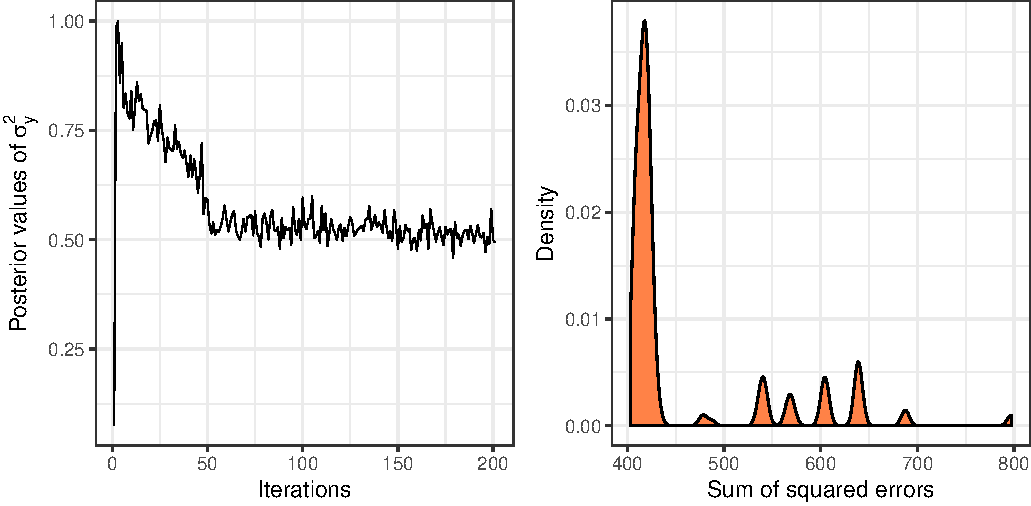
\includegraphics{how_to_use_files/figure-latex/unnamed-chunk-4-1} 

}

\caption{Chain for $\sigma^{2}$ and density of sum of squared errors for a B-CART model run with 200 iterations}\label{fig:unnamed-chunk-4}
\end{figure}

\begin{Shaded}
\begin{Highlighting}[]
\CommentTok{# Using the prediction function }
\NormalTok{test <-}\StringTok{ }\NormalTok{data }\OperatorTok\StringTok{ }\KeywordTok{filter}\NormalTok{(set }\OperatorTok{==}\StringTok{ "test"}\NormalTok{) }\OperatorTok\StringTok{ }\KeywordTok{select}\NormalTok{(}\OperatorTok{-}\NormalTok{set)}
\NormalTok{pred <-}\StringTok{ }\KeywordTok{predict_bcart}\NormalTok{(}\DataTypeTok{model =}\NormalTok{ bcart_model, }\DataTypeTok{newdata =}\NormalTok{ test)}

\NormalTok{pred }\OperatorTok\StringTok{ }
\StringTok{  }\KeywordTok{group_by}\NormalTok{(node) }\OperatorTok\StringTok{ }
\StringTok{  }\KeywordTok{summarise}\NormalTok{(}\DataTypeTok{ssr =} \KeywordTok{sum}\NormalTok{((y }\OperatorTok{-}\StringTok{ }\NormalTok{prediction)}\OperatorTok{^}\DecValTok{2}\NormalTok{),}
            \DataTypeTok{mean_of_y =} \KeywordTok{mean}\NormalTok{(y), }
            \DataTypeTok{mu_prediction =} \KeywordTok{mean}\NormalTok{(prediction))}
\end{Highlighting}
\end{Shaded}

\begin{verbatim}
## # A tibble: 18 x 4
##    node                                         ssr mean_of_y mu_prediction
##    <chr>                                      <dbl>     <dbl>         <dbl>
##  1 root X2 left X5 left X4 left X3 left       4.08     1.33         1.32   
##  2 root X2 left X5 left X4 left X3 right X2~  0.699    2.49         1.66   
##  3 root X2 left X5 left X4 left X3 right X2~  1.22     2.96         1.86   
##  4 root X2 left X5 left X4 right X1 left X5~ 10.8      1.14         0.815  
##  5 root X2 left X5 left X4 right X1 left X5~  0.530    0.172       -0.0779 
##  6 root X2 left X5 left X4 right X1 left X5~  1.01     0.516        1.03   
##  7 root X2 left X5 left X4 right X1 left X5~  1.08     1.05         0.480  
##  8 root X2 left X5 left X4 right X1 left X5~  4.59     0.113        0.612  
##  9 root X2 left X5 left X4 right X1 right     8.91     0.126        0.00270
## 10 root X2 left X5 right X4 left X1 left X2~  8.93     0.717        0.734  
## 11 root X2 left X5 right X4 left X1 left X2~  1.28     0.782        0.788  
## 12 root X2 left X5 right X4 left X1 left X2~  0.801    0.0348       0.0952 
## 13 root X2 left X5 right X4 left X1 left X2~  0.278    0.637        0.573  
## 14 root X2 left X5 right X4 left X1 right    15.8     -0.168       -0.202  
## 15 root X2 left X5 right X4 right            16.0     -0.609       -0.676  
## 16 root X2 right X4 left                      2.93     0.288       -0.0707 
## 17 root X2 right X4 right X2 left            19.9     -0.686       -0.697  
## 18 root X2 right X4 right X2 right            5.88    -1.12        -1.07
\end{verbatim}

\hypertarget{regex-dictionary}{%
\subsection{Regex dictionary}\label{regex-dictionary}}

Some regular expression were used in the pruning part of the model. They
can be described as:

\begin{itemize}
\tightlist
\item
  \texttt{\textquotesingle{}(\ right\textbar{}\ left)\$\textquotesingle{}}:
  detects the last ``right'' or ``left'';
\item
  \texttt{\textquotesingle{}X{[}0-9{]}{[}\^{}X{[}0-9{]}{]}*\$\textquotesingle{}}:
  detects the last X followed by a number;
\item
  \texttt{\textquotesingle{}(?\textless{}=\textquotesingle{}something\textquotesingle{}\textbackslash{}\textbackslash{}s).*\textquotesingle{}}:
  detects everything after the ``something'';
\item
  \texttt{\textquotesingle{}(\ X{[}0-9{]}\ right\textbar{}\ X{[}0-9{]}\ left)\$\textquotesingle{}}:
  detects the last X followed by a number and a ``left'' or ``right'';
\end{itemize}

\hypertarget{refs}{}
\leavevmode\hypertarget{ref-Friedman1991}{}%
Friedman, Jerome H. 1991. ``Rejoinder: Multivariate Adaptive Regression
Splines.'' \emph{The Annals of Statistics}.
\url{https://doi.org/10.1214/aos/1176347973}.


\end{document}
